%!TEX root = ../draft.tex

\section{Empirical Analysis}
\label{sec:Analysis}

In this section, we begin by describing six large-scale network datasets that we
use in our analysis and experiments. Then, we describe global network properties,
insights from empirical studies in the Social Science and common assumptions in
network modeling. Finally, we discuss the role of structural proximity in edge
formation.

\subsection{Datasets}
\label{sec:Datasets}

We consider six citation networks of different scales (size, time) from diverse
sources: research articles, utility patents and judicial cases. We list the
summary statistics and global network properties of these datasets in~\Cref{table:datasets}.
Three of the six datasets are attributed networks; that is, each node has a categorical attribute value.

We focus on citation networks for two reasons. First, since nodes in citation networks form
all outgoing edges to existing nodes at the time of joining the network,
citation networks provide a clean basis to study edge formation mechanisms in
attributed social networks. Second, citation network span long periods of time (e.g.,
the \texttt{USSC} judicial citation network span several hundred years).
As a result, identifying local edge formation processes that accurately model
growth for this duration is non-trivial. Next, we study the structural and content
properties of these networks.

% Now, we briefly describe the datasets considered in this paper.
% \Cref{table:datasets} provides summary statistics of the following networks:
% \begin{enumerate}
%     % (V,E) = (22049, 138871), used (V,E): 18665 115358
%     \item{\textbf{Association of Computational Linguistics}} (\texttt{ACL}) \cite{acldata} is an attributed academic citation network
%     that consists of papers published in ACL conferences, journals and workshops.
%     The attribute value of each paper is the name of the venue where it was published.
%
%     % (V,E) = (22049, 138871), used (V,E): 18665 115358
%     % \item{\textbf{Python Package Index}} (\texttt{PYPI}) \footnote{http://web.stanford.edu/class/cs224w/resources.html} is an attributed dependency graph of Python
%     % software packages. Each software package is associated with a category.
%
%     % entire dataset used
%     \item{\textbf{U.S. Supreme Court Cases}} (\texttt{USSC}) \cite{fowler2008authority} is a judicial citation network of
%     U.S. Supreme Court cases. There is an edge from case $i$ to case $j$ if and only if case $i$ cites case $j$ in its majority opinion.
%
%     % used: (V,E) = (30,558, 347,228) after removing nodes w. missing time data
%     \item{\textbf{ArXiv HEP-PH}} (\texttt{HEP-PH}) \cite{gehrke2003overview} is an academic citation network of HEP-PH (high energy
%     physics phenomenology) papers in the ArXiv e-print.
%
%     % used: (V,E) = (556661, 6647769) after removing nodes w. missing time + categorial data
%     \item{\textbf{APS Journals}} (\texttt{APS}) is an attributed academic citation network maintained by
%     the American Physical Society (\texttt{APS}).
%     The attribute value of each paper is the \texttt{APS} journal in which it was published.
%
%     % used: (V,E) = (2047881, 10088564) after removing nodes w. missing time + categorical data
%     \item{\textbf{U.S Utility Patents}} (\texttt{Patents}) \cite{leskovec2005graphs} is an attributed citation network of U.S. utility patents maintained by
%     the National Bureau of Economic Research (NBER).
%     The attribute value of each patent is an NBER patent category.
%
%     % used: (V,E) = (5987642, 45028807) after removing nodes w. missing time data
%     \item{\textbf{Semantic Scholar}} (\texttt{Semantic}) \cite{ammar} is an academic citation network of
%     Computer Science and Neuroscience papers, released in June 2017 by Semantic Scholar.
% \end{enumerate}

% in \cref{subsec:factors} and empirically
% validate the effectiveness of the proposed model using these network datasets in~\Cref{sec:Experiments}.
%
% In this section, we outlined the citation network datasets that we use in our analysis and experiments.
% Next, we discuss common factors that affect edge formation mechanisms and identify common global structural
% properties of real networks.


\subsection{Global Network Properties}
\label{subsec:factors}

% Factors that influence edge formation at the nodal level have a cumulative
% effect on global structural properties of real-world networks.
Compact statistical descriptors of global network properties ~\cite{newman2010networks}
such as degree distribution, local clustering, and attribute assortativity
quantify the extent to which local edge formation phenomena shape global network
structure.

\textbf{Heavy tailed degree distribution:}
Real-world networks tend to exhibit heavy tailed degree distributions.
These distributions can emerge from the well-known preferential attachment
process~\cite{simon1955class,barabasi1999emergence}, where incoming nodes
connect with nodes in proportion to their degree.
% Over time, preferential
% attachment amplifies initial differences in node degree, giving rise to heavy tailed
% distributions.
% (also known as the ``rich get richer'' effect) in citation networks; It also implies that most papers receive zero or a few
% citations, but a small but significant percent of the nodes turn into popular
% hubs that receive many citations.
Log-normal fits, with parameters listed in~\Cref{table:netstats}, well describe
the in-degree distribution of all network datasets, consistent Broido and
Clauset's~\cite{broido2018scale} observation that scale-free, real-world networks
are rare
% with truly
% power law degree distributions are rare.
% Our model explains the emergence of heavy tailed in-degree distributions through a
% \textit{local} process that adjusts bias towards linking to well-connected nodes

\begin{figure}[b]
 \vspace{-10pt}
 \centering
 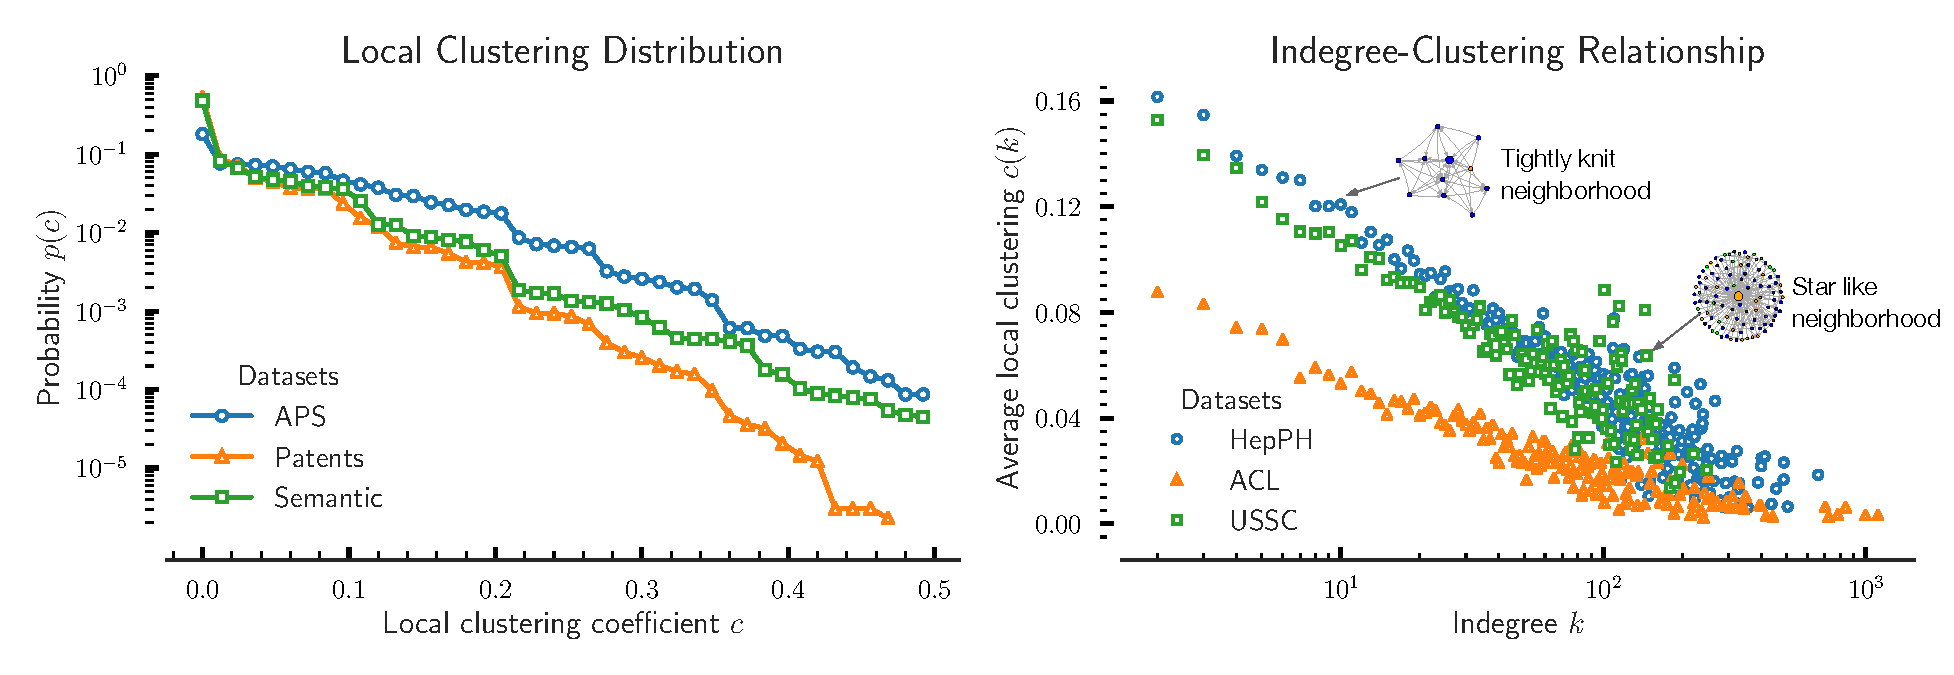
\includegraphics[width=\columnwidth]{clustering}
 \caption{
    Local clustering in real-world networks have common characteristics:
    skewed local clustering distribution (left subplot) and a negatively correlated
    relationship between in-degree and average local clustering (right subplot).
 }
 \label{fig:cc_dc}
 \vspace{-10pt}
\end{figure}

\textbf{High Local Clustering:}
Real-world networks exhibit high local clustering
(\texttt{LCC}), as shown in~\Cref{table:netstats}. Local
clustering can arise from triadic closure~\cite{simmel1950sociology,
newman2001clustering}, where nodes with common neighbor(s) have an increased
likelihood of forming a connection.
The coefficient of node $i$ equals the probability with which two randomly chosen
neighbors of the node $i$ are connected. In directed networks, the neighborhood
of a node $i$ can refer to the nodes that link to $i$, nodes that
$i$ links to or both. We define the neighborhood to be the set
of all nodes that link to node $i$. In ~\Cref{fig:cc_dc}, we show that (a) average local clustering is not a
representative statistic of the skewed local clustering distributions and (b) real-world networks
exhibit a negative correlation between in-degree and clustering.
That is, low in-degree nodes have small, tightly knit neighborhoods
and high in-degree nodes tend have large, star-shaped neighborhoods.
% Empirical studies
% \cite{kossinets2006empirical} show that the probability of edge formation
% increases with the number of common neighbors.
% The local clustering coefficient of a node measures the prevalence of triadic
% closure in its neighborhood.
% in~\Cref{fig:cc_dc}. Furthermore, real-world networks exhibit a negative
% correlation between node in-degree  and local clustering. In~\Cref{fig:cc_dc},
% we also observe that the average local clustering  decreases as in-degree
% increases.
% We propose a model
% that explains how clustering in real-world networks can arise from local processes
% of exploration \& link formation.


% Homophily and Assortativity
\textbf{Homophily:}
Attributed networks tend to exhibit homophily~\cite{mcpherson2001birds}, the
phenomenon where similar nodes are more likely to be connected than dissimilar
nodes. The assortativity coefficient ~\cite{newman2002assortative} $r \in [-1,
1]$, quantifies the level of homophily in an attributed network.
%  and indicates
% the extent to which attribute similarity influences edge formation.
Intuitively,
assortativity compares the observed fraction of edges between nodes with the same attribute
value to the expected fraction of edges between nodes with same attribute value
if the edges were rewired randomly. In~\Cref{fig:mixing}, we show that
attributed networks \texttt{ACL}, \texttt{APS} and \texttt{Patents} exhibit
varying level of homophily with assortativity coefficient ranging from $0.07$ to
$0.72$.

% We embed attribute based preferences at the local level lead to generate networks
% with varying attribute mixing patterns.

\begin{figure}
 \centering
 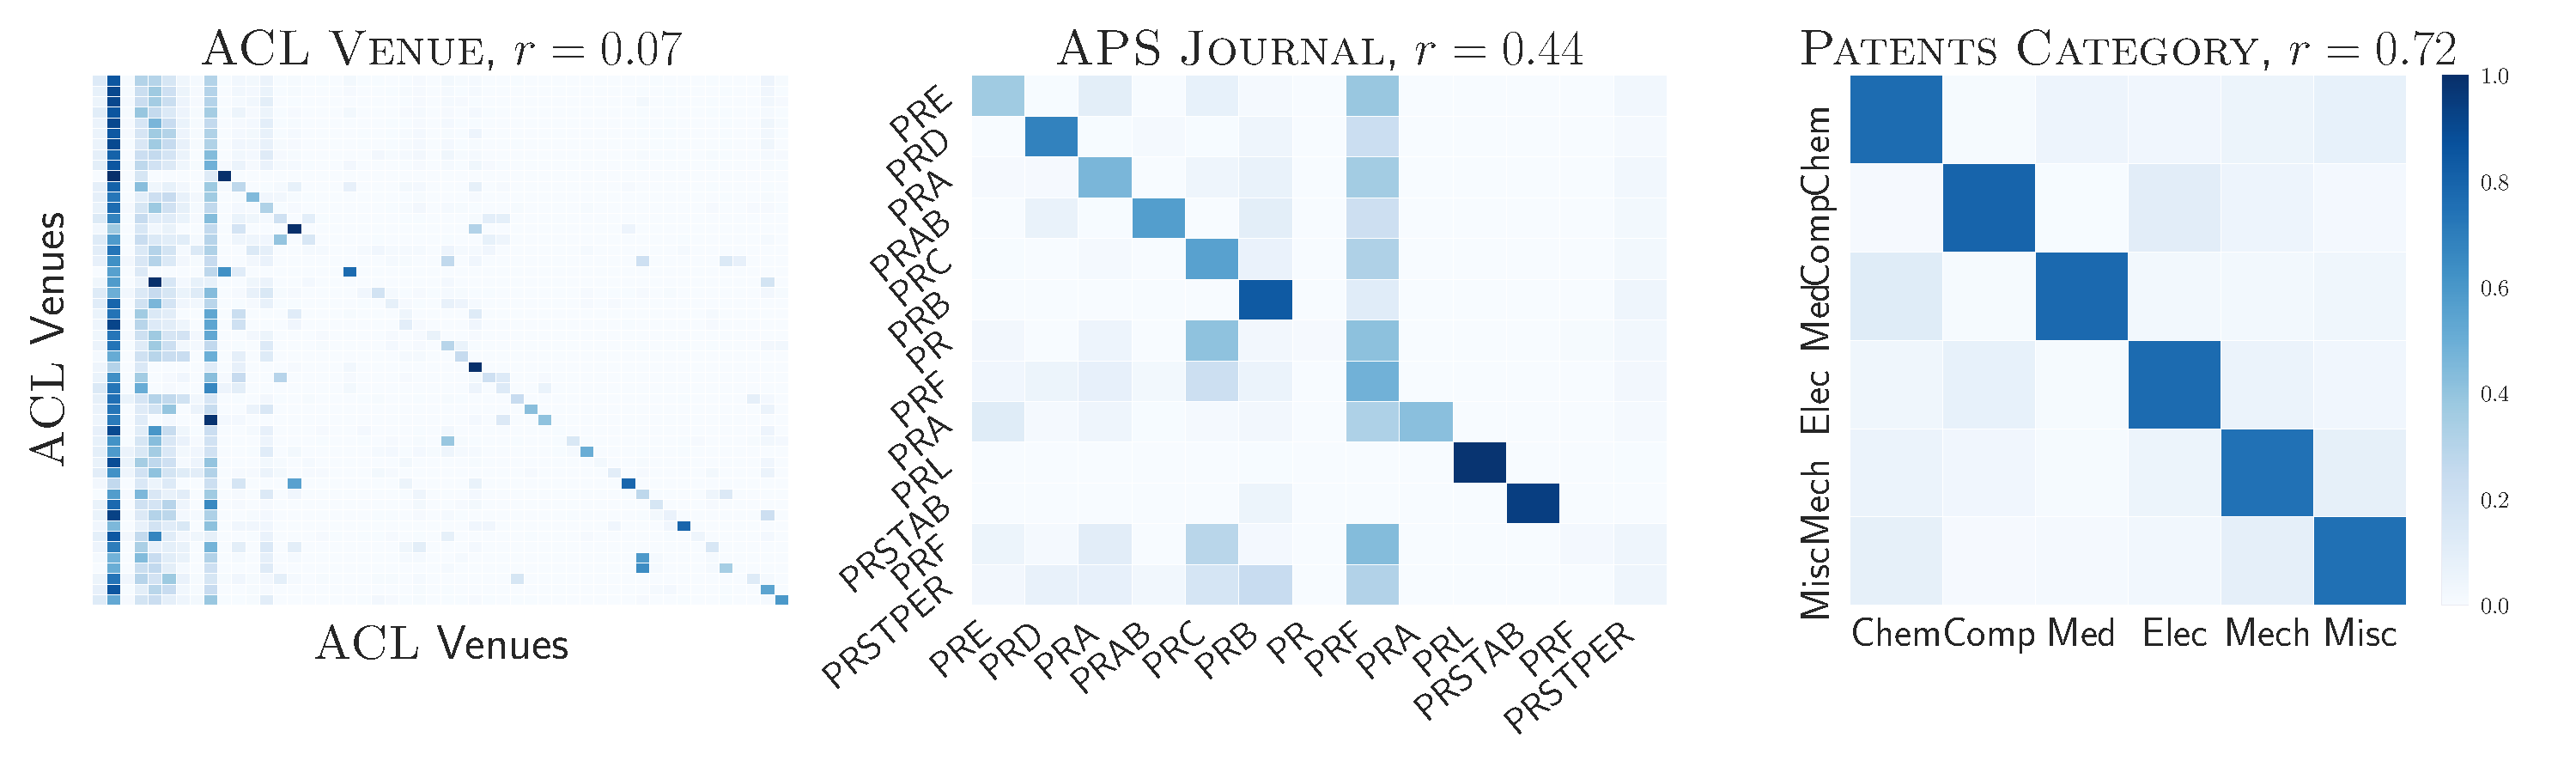
\includegraphics[width=\columnwidth]{homophily}
 \caption{
    Attributed networks exhibit varying levels of homophily. The subplots
    illustrate the mixing patterns in \texttt{ACL}, \texttt{APS} and \texttt{Patents}
    w.r.t. attributes \texttt{Venue} ($r=0.07$), \texttt{Journal} ($r=0.44$) and
    \texttt{Category} ($r=0.72$) respectively.
 }
 \label{fig:mixing}
 \vspace{-20pt}
\end{figure}

\textbf{Increasing Out-degree over Time:}
The out-degree of nodes that join real-world networks tends to increase as
functions of network size and time. This phenomenon densifies networks and
can shrink effective diameter over time. Densification tends to exhibit a power law
relationship ~\cite{leskovec2005graphs} between the number of edges $e(t)$ and
nodes $n(t)$ at time $t$: $e(t) \propto n(t)^{\alpha}$.~\Cref{table:netstats}
lists the densification power law (\texttt{DPL}) exponent $\alpha$ of the
network datasets.

To summarize, citation networks tend to be homophilic networks that undergo
accelerated network growth and exhibit regularities in structural properties:
heavy tailed in-degree distribution, skewed local clustering distribution,
negatively correlated degree-clustering relationship, and varying attribute
mixing patterns.

% In our proposed model, we increase the outdegree of incoming nodes at a linear
% or superlinear rate to account for the accelerated network growth observed in
% real networks.

% To summarize, factors such as preferential attachment, triadic closure and
% homophily not only influence how individuals form connections at the local level
% but also explain regularities arise in global structural properties of
% real-world networks. Next, we discuss empirical studies from sociology that
% examine network formation and decision making.

\subsection{Insights from Sociological Studies}

Sociological studies on network formation seek to explain
how individuals form edges in real-world networks.

\textbf{Interplay of Triadic Closure and Homophily:}
Empirical studies~\cite{35626,block2014multidimensional} that analyze the
interplay between triadic closure and homophily
 % in evolving networks
  indicate
that \textit{both} structural proximity and homophily are statistically
significant factors that simultaneously influence edge formation.
Homophilic preferences~\cite{mcpherson2001birds} induce edges between similar
nodes, whereas structural factors such as network distance limit
edge formation to proximate nodes (e.g. friend of a
friend).

\textbf{Bounded Rationality:}
Extensive work~\cite{simon1972theories,gigerenzer1996reasoning,lipman1995information} on
decision making shows that individuals are boundedly rational
actors; constraints such as limited information, cognitive capacity and time impact decision making.
This suggests that resource-constrained individuals that join networks are likely to employ simple rules
to form edges using limited information and partial network access.
% For example, a researcher cites academic
% papers without knowledge of, or access to, the entire literature in her field.

Current preferential attachment and fitness-based models
\cite{dorogovtsev2000structure,singh2017relay,barabasi1999emergence}
make two assumptions that are at variance with these findings.
First, by assuming that successive edge formations are independent,
these models disregard the effect of triadic closure and structural proximity.
Second, these models implicitly require incoming nodes to have complete network
access (e.g., be able to connect to any node) or explicit knowledge of one or
more properties (e.g., fitness, degree) of every node. For
example, a preferential attachment model, by making connections in proportion to
degree, requires non-local information: the degree distribution of the entire
network.

To summarize, insights from sociological studies indicate that edge formation in real-world
networks comprises biases towards nodes that are similar, well-connected or
structurally proximate. Next, we analyze the role of structural proximity in edge
formation.

\subsection{Proximity-biased Edge Formation}

We investigate the effect of structural proximity on edge formation in real-world networks.
Prior work~\cite{35626} shows that the probability of edge formation in social networks
decreases as a function of network distance.
Indeed, triadic closure explains how individuals form additional
edges to proximate nodes (e.g. friend of friend) over time.
However, we lack a concrete understanding of the extent to which structural
proximity influences edge formation in bibliographic networks, wherein incoming nodes form all edges at
the time of joining the network. In~\Cref{fig:locality}, we show high structural proximity
among incoming (shown in blue) node's (shown in red) connections in the \texttt{Hep-PH} dataset
hints at edge formation processes biased towards proximate nodes in the same local neighborhood.

% While prior work~\cite{35626} shows that the probability of
% edge formation in social networks decreases as a function of network distance,
% explained through processes like triadic closure, there are is a key difference
% with directed citation networks that we study. In social networks, edge
% formation can take place after the nodes join, whereas in citation networks, a
% node forms all edges at the time of joining. This means that probability of
% triadic closure changes over time. If nodes do not drop out, this probability
% increases with time. Thus in a citation network, it is unclear if one should
% expect if the set of nodes $\{k \}$ that a incoming node $i$ cites should be

% The left subplot in \Cref{fig:locality} shows high structural proximity between
% an incoming (shown in blue) node's  connections (shown in red) in the
% \texttt{Hep-PH} dataset. This hints at edge formation processes biased towards
% nodes in the same local neighborhood.

% Due to the unavailability of navigational data such as the sequence in which individuals form edges,

\begin{figure}[H]
%  \vspace{-4pt}
 \centering
 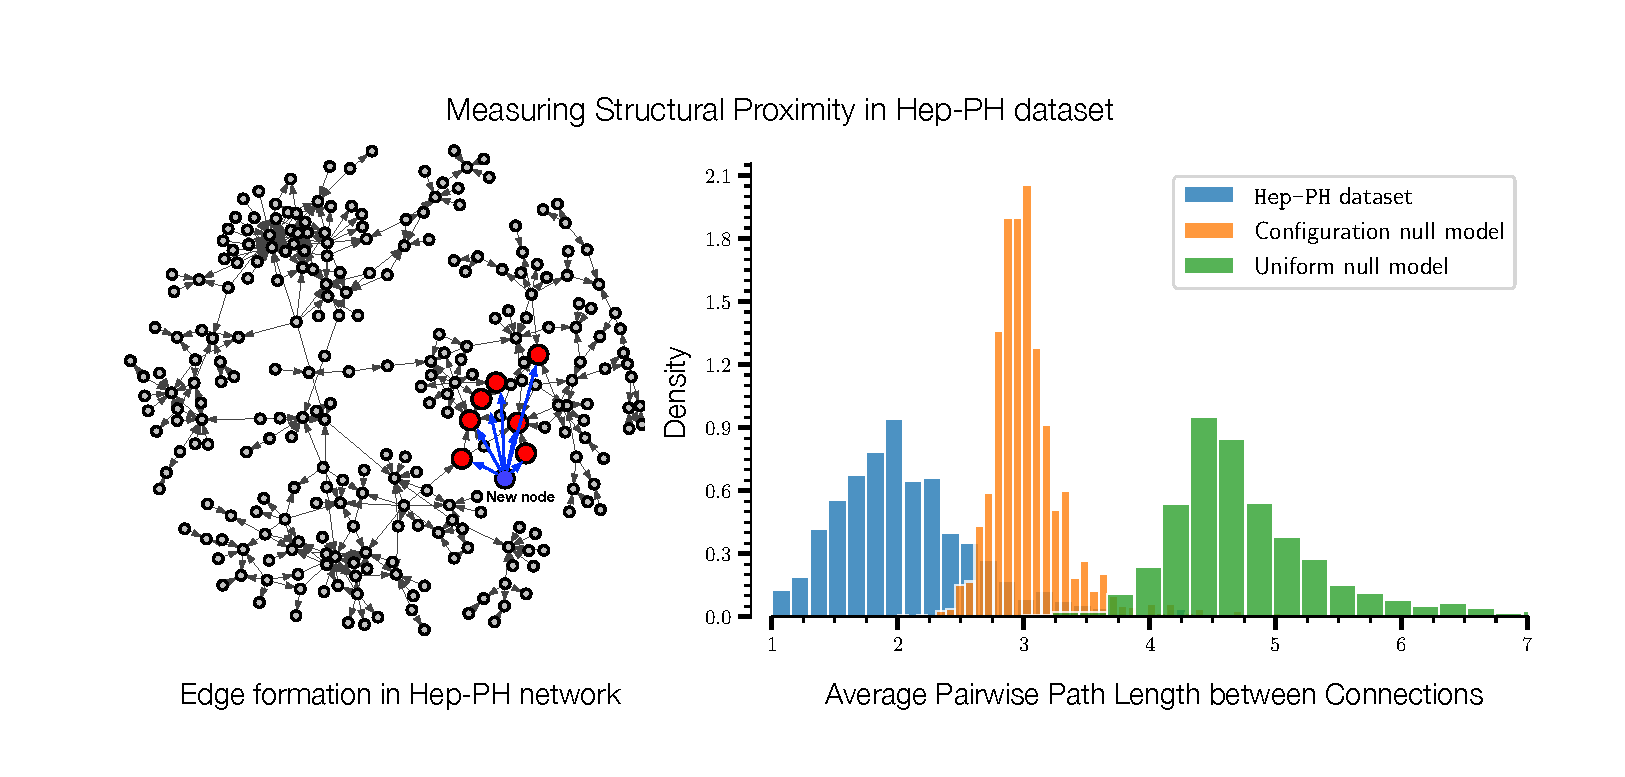
\includegraphics[width=\columnwidth]{locality_v4}
 \caption{
    Proximity-biased edge formation. The diagram and proximity distributions
    collectively indicate how edge formation in real-world networks are biased
    towards structurally proximate nodes in the same locality.  }
 \label{fig:locality}
 % \vspace{-10pt}
\end{figure}
We rely on network snapshots and
node arrival sequence to estimate a statistic based on path length that measures
structural proximity between nodes' connections. Consider an incoming node $u$ that forms edges to nodes in $N(u)$.
To measure the proximity between node $u$'s connections, we compute the average
pairwise shortest path distance between the connections in the network snapshot
immediately preceding node $u$'s arrival.


The right subplot in~\Cref{fig:locality} compares the proximity statistic
distribution of the \texttt{Hep-PH} dataset to two null models: uniform and
configuration. In the uniform model, incoming nodes form connections to existing
nodes uniformly at random, whereas the configuration model  randomly
rewire all edges in \texttt{Hep-PH} while preserving the out-degree and in-degree
distributions. We first observe that the connections of incoming nodes in the uniform
null model are structurally distant from each other on average.
Although the presence of hubs in the configuration model
considerably decreases the distance between nodes' connections, it does
not explain why the majority of connections in \texttt{Hep-PH} are either
connected directly or via an intermediate node. The disparity between the
observed and null distributions suggests that structural proximity between
connections is intrinsic to edge formation in real-world networks.




To summarize, empirical analyses and insights from the Social Sciences motivate
the need to model how resource-constrained edge formation processes collectively
shape well-defined global network properties of large-scale networks over time.
% Next, we propose a growth model that explains how local processes of
% edge formation can lead to the emergence of key global structural and
% attribute properties observed in real-world networks.



% citation networks tend to be homophilic networks that
% undergo accelerated network growth and exhibit regularities in structural
% properties: heavy tailed in-degree distribution, skewed local clustering distribution,
% negatively correlated degree-clustering relationship and varying attribute mixing patterns.
% These global properties are modulated by the presence of resource constrained edge formation decisions.
% and global structural properties can be better understood by studying network snapshots at different
% stages of the growth process.
% datasets include the time (e.g., publication year of academic papers) at which nodes join the network.
% As a result, local edge formation processes and global structural properties can be better understood by studying
% network snapshots at different stages of the growth process. Third, the citation networks are large networks that
% tend to have one or more nodal attributes (e.g. category of patents)
% and span multiple decades. As a result, the structural and content properties of the citation
% networks considered are well-defined.

% Nodes do
% not form or delete edges at a later time. This allows us to analyze
% the edge formation mechanisms of new nodes that join the network form edges.
% % Other edge dynamics such as edge deletion and addition of edges between existing
% % nodes are important and we plan to investigate them at a later time.
% Second, citation network datasets include the time (e.g., publication year of academic
% papers) at which nodes join the network. As a result, local edge formation
% processes and global structural properties can be better understood by studying
% network snapshots at different stages of the growth process. Third, the citation
% networks are large networks that tend to have one or more nodal attributes (e.g. category of patents)
% and span multiple decades. As a result, the structural and content properties of the citation
% networks considered are well-defined.

% \begin{table}[b]
%  \center
%  {
%   \begin{tabular}[c]{lrrrr} \toprule
%   Network Dataset &  \texttt{LN} $(\mu, \sigma)$ & \texttt{DPL} $\alpha$       &  Avg. ${\texttt{LCC}}$  & \texttt{AA} $r$   \\ \midrule
%   \texttt{USSC}     &   (1.19, 1.18) & 2.32     & 0.12    & -     \\
%   \texttt{HEP-PH}   &   (1.32, 1.41) & 1.67     & 0.12    & -     \\
%   \texttt{Semantic} &   (1.78, 0.96)  & 1.58     & 0.06    & -     \\   \midrule
%   \texttt{ACL}      &   (1.93, 1.38)  & 1.43     & 0.07    & 0.07     \\
%   \texttt{APS}      &   (1.62, 1.20)  & 1.26     & 0.11    & 0.44     \\
%   \texttt{Patents}  &   (1.10, 1.01)   & 1.94     & 0.04    & 0.72    \\
%   % \texttt{PYPI}         & 1.208     & 0.0524    & 0.692   & a\\
%    \bottomrule
%   \end{tabular}
%   \vspace{1mm}
%   \caption{Global network properties: lognormal (\texttt{LN}) in-degree distribution mean and standard deviation $(\mu, \sigma)$,
%   densification power law (\texttt{DPL}) exponent $\alpha$, average local clustering coefficient (${\texttt{LCC}}$)
%   and attribute assortativity (\texttt{AA}) coefficient of six network datasets.}
%   \label{table:netstats}
%  }
% \end{table}

